% answers.tex —— 2010 年·普通高等学校招生考试·天津卷·文科 · 参考答案与详细解析片段
% 由 tools/generate_projects.py 依来源总账自 2010/2010_数学真题_天津文_试题.md + 2010/2010_数学真题_天津文_解析正文.md + 2010/2010_数学真题_天津文_答案要点.md 生成，勿手改（改源 MD 后重跑）


\begin{gktip}
固定候选 PDF 仅含题面，无答案、解析和评分标准，原页亦未标分值；以下为非官方编者独立推导，官方答案字段为空。分数、根号、上下标与六幅图均以 600 dpi 原页复核。第 3 题依上游勘误版题面（运行程序求输出）作答，原固定件同题题面与框图矛盾，详见 \texttt{ISSUE-1523}。
\end{gktip}

\begin{answer}
\gksolhead{1}{}

\textbf{题目}：

$i$ 是虚数单位，复数 $\dfrac{3+i}{1-i}=$（　）

（A）$1+2i$

（B）$2+4i$

（C）$-1-2i$

（D）$2-i$

\Needspace{4\baselineskip}
\textbf{解析}

\nopagebreak[4]
\[\frac{3+i}{1-i}=\frac{(3+i)(1+i)}{(1-i)(1+i)}
=\frac{2+4i}2=1+2i.\]

\gkanswer{答案：A。}

\end{answer}
\begin{answer}
\gksolhead{2}{}

\textbf{题目}：

设变量 $x,y$ 满足约束条件 $\begin{cases}x+y\leqslant3,\\ x-y\geqslant-1,\\ y\geqslant1,\end{cases}$ 则目标函数 $z=4x+2y$ 的最大值为（　）

（A）$12$

（B）$10$

（C）$8$

（D）$2$

\Needspace{4\baselineskip}
\textbf{解析}

\Needspace{5\baselineskip}
可行域的三个顶点为 $(2,1)$、$(0,1)$、$(1,2)$，对应

\nopagebreak[4]
\[z=4x+2y=10,\ 2,\ 8.\]

最大值为 $10$。

\gkanswer{答案：B。}

\end{answer}
\begin{answer}
\gksolhead{3}{}

\textbf{题目}：

阅读下面的程序框图，运行相应的程序，则输出 $s$ 的值为（　）
\nopagebreak[4]
\begin{center}% 2010 年天津卷文科第 3 题：程序框图，输出 s 的值。
% 来源 PDF：普通高考/2010/2010天津文.pdf（上游勘误版），SHA-256 e6b06813e17b7c332b651b8784c8fab0fcad0c8666ea6032a2958917c55307c9。
% 原页：第 1 页（A3 四栏）第 1 栏中部，书页码 637。
% 重绘依据：开始 → s=1 → i=1 → s=s(3−i)+1 → i=i+1 → 判断 i>4；
%   是（下）→ 输出 s → 结束；否（右）回到 s=s(3−i)+1 上方。
\begin{tikzpicture}[scale=0.66, semithick, >=Stealth,
  node distance=2.8mm, every node/.style={inner sep=2pt, font=\small}]
  \node (start) [draw, rounded corners=4pt, minimum width=1.7cm, minimum height=0.52cm] {开始};
  \node (init) [draw, minimum width=1.7cm, minimum height=0.52cm, below=of start] {$s=1$};
  \node (idx) [draw, minimum width=1.7cm, minimum height=0.52cm, below=of init] {$i=1$};
  \node (step) [draw, minimum width=4.3cm, minimum height=0.52cm, below=of idx] {$s=s\cdot(3-i)+1$};
  \node (inc) [draw, minimum width=1.9cm, minimum height=0.52cm, below=of step] {$i=i+1$};
  \node (cond) [draw, diamond, aspect=1.9, minimum width=2.2cm, minimum height=0.8cm, below=of inc] {$i>4?$};
  \node (out) [draw, trapezium, trapezium left angle=70, trapezium right angle=110,
    minimum width=2.2cm, minimum height=0.52cm, below=of cond] {输出 $s$};
  \node (end) [draw, rounded corners=4pt, minimum width=1.7cm, minimum height=0.52cm, below=of out] {结束};
  \draw[->] (start) -- (init);
  \draw[->] (init) -- (idx);
  \draw[->] (idx) -- (step);
  \draw[->] (step) -- (inc);
  \draw[->] (inc) -- (cond);
  \draw[->] (cond) -- (out);
  \node[anchor=west] at ($(cond.south)!0.5!(out.north)+(10pt,-2pt)$) {是};
  \draw[->] (cond.east) -- ++(0.8,0) |- node[pos=0.25, right] {否} (step.north);
  \draw[->] (out) -- (end);
\end{tikzpicture}
\end{center}
\nopagebreak[4]
（A）$-1$

（B）$0$

（C）$1$

（D）$3$

\Needspace{4\baselineskip}
\textbf{解析}

\Needspace{5\baselineskip}
初值 $s=1$，$i=1$。依次执行 $s=s(3-i)+1$：

\nopagebreak[4]
\[i=1:\ s=3;\quad i=2:\ s=4;\quad i=3:\ s=1;\quad i=4:\ s=0.\]

此时 $i=5>4$，输出 $s=0$。

\gkanswer{答案：B。}

\end{answer}
\begin{answer}
\gksolhead{4}{}

\textbf{题目}：

函数 $f(x)=\mathrm e^x+x-2$ 的零点所在的一个区间是（　）

（A）$(-2,-1)$

（B）$(-1,0)$

（C）$(0,1)$

（D）$(1,2)$

\Needspace{4\baselineskip}
\textbf{解析}

$f(0)=1+0-2=-1<0$，$f(1)=\mathrm e+1-2=\mathrm e-1>0$，且 $f$ 在 $\mathbf R$ 上单调递增，故零点在 $(0,1)$。

\gkanswer{答案：C。}

\end{answer}
\begin{answer}
\gksolhead{5}{}

\textbf{题目}：

下列命题中，真命题是（　）

（A）$\exists m\in\mathbf R$，使函数 $f(x)=x^2+mx$（$x\in\mathbf R$）是偶函数

（B）$\exists m\in\mathbf R$，使函数 $f(x)=x^2+mx$（$x\in\mathbf R$）是奇函数

（C）$\forall m\in\mathbf R$，使函数 $f(x)=x^2+mx$（$x\in\mathbf R$）是偶函数

（D）$\forall m\in\mathbf R$，使函数 $f(x)=x^2+mx$（$x\in\mathbf R$）是奇函数

\Needspace{4\baselineskip}
\textbf{解析}

$f(x)=x^2+mx$ 为偶函数当且仅当 $m=0$，故（A）真；含 $x^2$ 项的函数不可能为奇函数，故（B）（D）假；$m\neq0$ 时不是偶函数，故（C）假。

\gkanswer{答案：A。}

\end{answer}
\begin{answer}
\gksolhead{6}{}

\textbf{题目}：

设 $a=\log_54$，$b=(\log_53)^2$，$c=\log_45$，则（　）

（A）$a<c<b$

（B）$b<c<a$

（C）$a<b<c$

（D）$b<a<c$

\Needspace{4\baselineskip}
\textbf{解析}

$0<\log_53<\log_54<1$，故 $b=(\log_53)^2<\log_53<\log_54=a$；又 $c=\log_45>1$。所以 $b<a<c$。

\gkanswer{答案：D。}

\end{answer}
\begin{answer}
\gksolhead{7}{}

\textbf{题目}：

设集合 $A=\{x\mid|x-a|<1,x\in\mathbf R\}$，$B=\{x\mid1<x<5,x\in\mathbf R\}$。

若 $A\cap B=\varnothing$，则实数 $a$ 的取值范围是（　）

（A）$\{a\mid0\leqslant a\leqslant6\}$

（B）$\{a\mid a\leqslant2\text{ \text{或} }a\geqslant4\}$

（C）$\{a\mid a\leqslant0\text{ \text{或} }a\geqslant6\}$

（D）$\{a\mid2\leqslant a\leqslant4\}$

\Needspace{4\baselineskip}
\textbf{解析}

$A=(a-1,a+1)$。$A\cap B=\varnothing$ 等价于 $a+1\leqslant1$ 或 $a-1\geqslant5$，即 $a\leqslant0$ 或 $a\geqslant6$。

\gkanswer{答案：C。}

\end{answer}
\begin{answer}
\gksolhead{8}{}

\textbf{题目}：

如图是函数 $y=A\sin(\omega x+\varphi)$（$x\in\mathbf R$）在区间 $\left[-\dfrac\pi6,\dfrac{5\pi}6\right]$ 上的图象，为了得到这个函数的图象，只要将 $y=\sin x$（$x\in\mathbf R$）的图象上所有的点（　）
\nopagebreak[4]
\begin{center}% 2010 年天津卷文科第 8 题：区间 [−π/6, 5π/6] 上的 y=A sin(ωx+φ) 图象。
% 来源 PDF：普通高考/2010/2010天津文.pdf（上游勘误版），SHA-256 e6b06813e17b7c332b651b8784c8fab0fcad0c8666ea6032a2958917c55307c9。
% 原页：第 1 页（A3 四栏）第 2 栏上部，书页码 637。
% 重绘依据：曲线过 (−π/6,0)、(π/3,0)、(5π/6,0)，在 π/12 取最大值 1，在 7π/12 取最小值 −1。
\begin{tikzpicture}[semithick, x=2.4cm, y=1.5cm, every node/.style={inner sep=1.2pt, font=\small}]
  \draw[-stealth] (-0.62,0) -- (3.0,0) node[below] {$x$};
  \draw[-stealth] (0,-1.35) -- (0,1.45) node[left] {$y$};
  \node[below left] at (0,0) {$O$};
  \draw[thick,domain=-0.5236:2.6180,samples=160] plot (\x,{sin(2*\x r + pi/3 r)});
  \draw[dashed] (0,-1) -- (1.5,-1);
  \draw (-0.5236,0.04) -- (-0.5236,-0.04) node[below left] {$-\dfrac\pi6$};
  \draw (1.0472,0.04) -- (1.0472,-0.04) node[below] {$\dfrac\pi3$};
  \draw (2.6180,0.04) -- (2.6180,-0.04) node[below] {$\dfrac{5\pi}6$};
  \draw (-0.04,1) -- (0.04,1) node[left] {$1$};
  \draw (-0.04,-1) -- (0.04,-1) node[left] {$-1$};
\end{tikzpicture}
\end{center}
\nopagebreak[4]
（A）向左平移 $\dfrac\pi3$ 个单位长度，再把所得各点的横坐标缩短到原来的 $\dfrac12$ 倍，纵坐标不变

（B）向左平移 $\dfrac\pi3$ 个单位长度，再把所得各点的横坐标伸长到原来的 $2$ 倍，纵坐标不变

（C）向左平移 $\dfrac\pi6$ 个单位长度，再把所得各点的横坐标缩短到原来的 $\dfrac12$ 倍，纵坐标不变

（D）向左平移 $\dfrac\pi6$ 个单位长度，再把所得各点的横坐标伸长到原来的 $2$ 倍，纵坐标不变

\Needspace{4\baselineskip}
\textbf{解析}

\Needspace{5\baselineskip}
由图，半个周期为 $\dfrac\pi3-\left(-\dfrac\pi6\right)=\dfrac\pi2$，故周期 $T=\pi$，$\omega=2$；又 $x=-\dfrac\pi6$ 时 $y=0$ 且随后递增，取 $\varphi=\dfrac\pi3$。于是

\nopagebreak[4]
\[y=\sin\left(2x+\frac\pi3\right)=\sin\left[2\left(x+\frac\pi6\right)\right].\]

故向左平移 $\dfrac\pi6$ 后，再把横坐标缩短到原来的 $\dfrac12$ 倍。

\gkanswer{答案：C。}

\end{answer}
\begin{answer}
\gksolhead{9}{}

\textbf{题目}：

如图，在 $\triangle ABC$ 中，$AD\perp AB$，$\overrightarrow{BC}=\sqrt3\overrightarrow{BD}$，$|\overrightarrow{AD}|=1$，则 $\overrightarrow{AC}\cdot\overrightarrow{AD}=$（　）
\nopagebreak[4]
\begin{center}% 2010 年天津卷文科第 9 题：三角形 ABC 中 AD⊥AB，D 在 BC 上。
% 来源 PDF：普通高考/2010/2010天津文.pdf（上游勘误版），SHA-256 e6b06813e17b7c332b651b8784c8fab0fcad0c8666ea6032a2958917c55307c9。
% 原页：第 1 页（A3 四栏）第 2 栏中部，书页码 637。
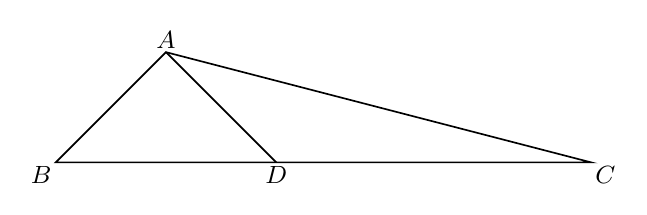
\begin{tikzpicture}[semithick, every node/.style={inner sep=1.2pt, font=\small}]
  \coordinate (A) at (-1.2,1.4);
  \coordinate (B) at (-2.6,0);
  \coordinate (D) at (0.2,0);
  \coordinate (C) at (4.2,0);
  \draw (A) -- (B) -- (C) -- cycle;
  \draw (A) -- (D);
  \node[above] at (A) {$A$};
  \node[below left] at (B) {$B$};
  \node[below] at (D) {$D$};
  \node[below right] at (C) {$C$};
\end{tikzpicture}
\end{center}
\nopagebreak[4]
（A）$2\sqrt3$

（B）$\dfrac{\sqrt3}2$

（C）$\dfrac{\sqrt3}3$

（D）$\sqrt3$

\Needspace{4\baselineskip}
\textbf{解析}

\Needspace{5\baselineskip}
取 $A(0,0)$，$D(1,0)$，$B(0,-b)$。由 $\overrightarrow{BC}=\sqrt3\overrightarrow{BD}$ 得

\nopagebreak[4]
\[C=B+\sqrt3(D-B)=(\sqrt3,\ b(\sqrt3-1)).\]

\Needspace{5\baselineskip}
故

\nopagebreak[4]
\[\overrightarrow{AC}\cdot\overrightarrow{AD}=\sqrt3\cdot1+0=\sqrt3.\]

\gkanswer{答案：D。}

\end{answer}
\begin{answer}
\gksolhead{10}{}

\textbf{题目}：

\Needspace{5\baselineskip}
设函数 $g(x)=x^2-2$（$x\in\mathbf R$），

\nopagebreak[4]
\[f(x)=\begin{cases}g(x)+x+4,&x<g(x),\\ g(x)-x,&x\geqslant g(x).\end{cases}\]

则 $f(x)$ 的值域是（　）

（A）$\left[-\dfrac94,0\right]\cup(1,+\infty)$

（B）$[0,+\infty)$

（C）$\left[-\dfrac94,+\infty\right)$

（D）$\left[-\dfrac94,0\right]\cup(2,+\infty)$

\Needspace{4\baselineskip}
\textbf{解析}

\Needspace{5\baselineskip}
$x<g(x)$ 即 $x^2-x-2>0$，得 $x<-1$ 或 $x>2$。此时

\nopagebreak[4]
\[f(x)=x^2+x+2=\left(x+\frac12\right)^2+\frac74,\]

值域为 $(2,+\infty)$。

\Needspace{5\baselineskip}
$x\geqslant g(x)$ 即 $-1\leqslant x\leqslant2$，此时

\nopagebreak[4]
\[f(x)=x^2-x-2=\left(x-\frac12\right)^2-\frac94,\]

值域为 $\left[-\dfrac94,0\right]$。

故 $f(x)$ 的值域为 $\left[-\dfrac94,0\right]\cup(2,+\infty)$。

\gkanswer{答案：D。}

\end{answer}
\begin{answer}
\gksolhead{11}{}

\textbf{题目}：

如图，四边形 $ABCD$ 是圆 $O$ 的内接四边形，延长 $AB$ 和 $DC$ 相交于点 $P$。若 $PB=1$，$PD=3$。

则 $\dfrac{BC}{AD}$ 的值为$\underline{\qquad}$。
\nopagebreak[4]
\begin{center}% 2010 年天津卷文科第 11 题：圆内接四边形 ABCD，AB 与 DC 延长交于 P。
% 来源 PDF：普通高考/2010/2010天津文.pdf（上游勘误版），SHA-256 e6b06813e17b7c332b651b8784c8fab0fcad0c8666ea6032a2958917c55307c9。
% 原页：第 1 页（A3 四栏）第 2 栏下部，书页码 637。
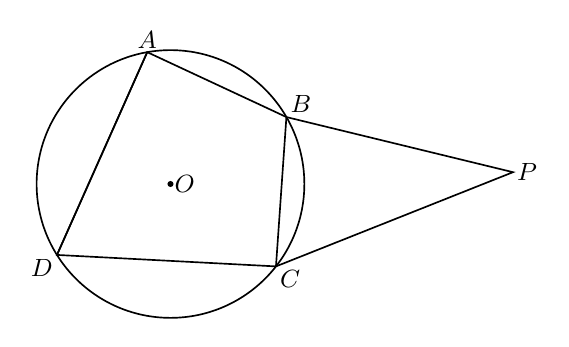
\begin{tikzpicture}[semithick, every node/.style={inner sep=1.2pt, font=\small}]
  \coordinate (O) at (0,0);
  \coordinate (A) at (100:1.7);
  \coordinate (B) at (30:1.7);
  \coordinate (C) at (-38:1.7);
  \coordinate (D) at (212:1.7);
  \coordinate (P) at (4.35,0.15);
  \draw (O) circle (1.7);
  \fill (O) circle (1.1pt);
  \node[right] at (O) {$O$};
  \draw (A) -- (B) -- (P) -- (C) -- (D) -- cycle;
  \draw (B) -- (C);
  \draw (A) -- (D);
  \node[above] at (A) {$A$};
  \node[above right] at (B) {$B$};
  \node[below right] at (C) {$C$};
  \node[below left] at (D) {$D$};
  \node[right] at (P) {$P$};
\end{tikzpicture}
\end{center}
\nopagebreak[4]
\Needspace{4\baselineskip}
\textbf{解析}

\Needspace{5\baselineskip}
四边形 $ABCD$ 内接于圆，故 $\angle PBC=\angle PDA$，$\angle PCB=\angle PAD$，于是 $\triangle PBC\sim\triangle PDA$。

\nopagebreak[4]
\[\frac{BC}{AD}=\frac{PB}{PD}=\frac13.\]

\gkanswer{答案：$\dfrac13$。}

\end{answer}
\begin{answer}
\gksolhead{12}{}

\textbf{题目}：

一个几何体的三视图如图所示，则这个几何体的体积为$\underline{\qquad}$。
\nopagebreak[4]
\begin{center}% 2010 年天津卷文科第 12 题：正视图、侧视图与俯视图。
% 来源 PDF：普通高考/2010/2010天津文.pdf（上游勘误版），SHA-256 e6b06813e17b7c332b651b8784c8fab0fcad0c8666ea6032a2958917c55307c9。
% 原页：第 1 页（A3 四栏）第 3 栏上部，书页码 637。
% 重绘依据：正视图为 2×1 矩形、中分；侧视图为 1×1 矩形；俯视图为梯形，上底 2、下底 1、高 2。
\begin{tikzpicture}[semithick, every node/.style={inner sep=1.2pt, font=\small}]
  % 正视图
  \draw (0,4.2) rectangle (2,5.2);
  \draw (1,4.2) -- (1,5.2);
  \node[below] at (1,3.7) {正视图};
  \draw[<->] (0,5.45) -- (1,5.45) node[midway,above] {$1$};
  \draw[<->] (1,5.45) -- (2,5.45) node[midway,above] {$1$};
  \draw[<->] (-0.4,4.2) -- (-0.4,5.2) node[midway,left] {$1$};
  % 侧视图
  \draw (3.4,4.2) rectangle (4.4,5.2);
  \node[below] at (3.9,3.7) {侧视图};
  \draw[<->] (3.4,5.45) -- (4.4,5.45) node[midway,above] {$1$};
  % 俯视图
  \draw (0,0) -- (1,0) -- (2,2) -- (0,2) -- cycle;
  \draw[<->] (0,-0.35) -- (1,-0.35) node[midway,below] {$1$};
  \draw[<->] (-0.4,0) -- (-0.4,2) node[midway,left] {$2$};
  \node[below] at (1.1,-0.95) {俯视图};
\end{tikzpicture}
\end{center}
\nopagebreak[4]
\Needspace{4\baselineskip}
\textbf{解析}

先求俯视图的面积。

\Needspace{5\baselineskip}
俯视图为梯形，上底 $2$、下底 $1$、高 $2$，面积

\nopagebreak[4]
\[S=\frac{2+1}2\times2=3.\]

正视图高为 $1$，故体积 $V=3\times1=3$。

\gkanswer{答案：$3$。}

\end{answer}
\begin{answer}
\gksolhead{13}{}

\textbf{题目}：

已知双曲线 $\dfrac{x^2}{a^2}-\dfrac{y^2}{b^2}=1$（$a>0$，$b>0$）的一条渐近线方程是 $y=\sqrt3x$，它的一个焦点与抛物线 $y^2=16x$ 的焦点相同。则双曲线的方程为$\underline{\qquad}$。

\Needspace{4\baselineskip}
\textbf{解析}

渐近线 $y=\sqrt3x$ 给出 $\dfrac ba=\sqrt3$。抛物线 $y^2=16x$ 的焦点为 $(4,0)$，故 $c=4$。由 $c^2=a^2+b^2=4a^2$ 得 $a^2=4$，$b^2=12$，双曲线为 $\dfrac{x^2}4-\dfrac{y^2}{12}=1$。

\gkanswer{答案：$\dfrac{x^2}4-\dfrac{y^2}{12}=1$。}

\end{answer}
\begin{answer}
\gksolhead{14}{}

\textbf{题目}：

已知圆 $C$ 的圆心是直线 $x-y+1=0$ 与 $x$ 轴的交点，且圆 $C$ 与直线 $x+y+3=0$ 相切。

则圆 $C$ 的方程为$\underline{\qquad}$。

\Needspace{4\baselineskip}
\textbf{解析}

\Needspace{5\baselineskip}
直线 $x-y+1=0$ 与 $x$ 轴交于 $(-1,0)$。圆心到 $x+y+3=0$ 的距离

\nopagebreak[4]
\[r=\frac{|-1+0+3|}{\sqrt2}=\sqrt2.\]

故圆的方程为 $(x+1)^2+y^2=2$。

\gkanswer{答案：$(x+1)^2+y^2=2$。}

\end{answer}
\begin{answer}
\gksolhead{15}{}

\textbf{题目}：

设 $\{a_n\}$ 是等比数列，公比 $q=\sqrt2$，$S_n$ 为 $\{a_n\}$ 的前 $n$ 项和。记 $T_n=\dfrac{17S_n-S_{2n}}{a_{n+1}}$，$n\in\mathbf N^*$。设 $T_{n_0}$ 为数列 $\{T_n\}$ 的最大项，则 $n_0=$ $\underline{\qquad}$。

\Needspace{4\baselineskip}
\textbf{解析}

\Needspace{5\baselineskip}
设首项为 $a_1$，则 $S_n=\dfrac{a_1(q^n-1)}{q-1}$，$a_{n+1}=a_1q^n$，故

\nopagebreak[4]
\[T_n=\frac{17(q^n-1)-(q^{2n}-1)}{(q-1)q^n}
=\frac{17-q^n-16q^{-n}}{q-1}.\]

令 $u=q^n=2^{n/2}>0$，则 $T_n$ 最大等价于 $u+\dfrac{16}u$ 最小，由均值不等式知 $u=4$ 时取最小，即 $2^{n/2}=4$，$n=4$。

\gkanswer{答案：$4$。}

\end{answer}
\begin{answer}
\gksolhead{16}{}

\textbf{题目}：

设函数 $f(x)=x-\dfrac1x$，对任意 $x\in[1,+\infty)$，$f(mx)+mf(x)<0$ 恒成立，则实数 $m$ 的取值范围是$\underline{\qquad}$。

\Needspace{4\baselineskip}
\textbf{解析}

\nopagebreak[4]
\[f(mx)+mf(x)=2mx-\frac{m+\frac1m}{x}<0\quad(x\geqslant1).\]

记 $g(x)=2mx-\dfrac{m+\frac1m}{x}$。

若 $m>0$，$g(x)$ 在 $[1,+\infty)$ 上递增且无上界，不可能恒负。

若 $m<0$，$g(x)$ 递减，只需 $g(1)=m-\dfrac1m<0$，即 $\dfrac{m^2-1}{m}<0$，由 $m<0$ 得 $m^2-1>0$，故 $m<-1$。

所以 $m\in(-\infty,-1)$。

\gkanswer{答案：$(-\infty,-1)$。}

\end{answer}
\begin{answer}
\gksolhead{17}{}

\textbf{题目}：

在 $\triangle ABC$ 中，$\dfrac{AC}{AB}=\dfrac{\cos B}{\cos C}$。

（1）证明：$B=C$；

（2）若 $\cos A=-\dfrac13$，求 $\sin\left(4B+\dfrac\pi3\right)$ 的值。

\Needspace{4\baselineskip}
\textbf{解析}

\Needspace{5\baselineskip}
（1）由正弦定理 $\dfrac{AC}{AB}=\dfrac{\sin B}{\sin C}$，结合已知得

\nopagebreak[4]
\[\frac{\sin B}{\sin C}=\frac{\cos B}{\cos C}
\Longrightarrow \sin B\cos C=\cos B\sin C
\Longrightarrow \sin(B-C)=0.\]

因 $B,C\in(0,\pi)$，故 $B=C$。

（2）由 $B=C$ 得 $2B=\pi-A$。又 $\cos A=-\dfrac13$，故 $\sin A=\dfrac{2\sqrt2}3$，$\cos2A=2\cos^2A-1=-\dfrac79$，$\sin2A=2\sin A\cos A=-\dfrac{4\sqrt2}9$。

\Needspace{5\baselineskip}
于是

\nopagebreak[4]
\[\sin\left(4B+\frac\pi3\right)
=\sin\left(2\pi-2A+\frac\pi3\right)
=\sin\left(\frac\pi3-2A\right),\]

\nopagebreak[4]
\[\sin\left(\frac\pi3-2A\right)
=\frac{\sqrt3}2\cos2A-\frac12\sin2A
=-\frac{7\sqrt3}{18}+\frac{2\sqrt2}9
=\frac{4\sqrt2-7\sqrt3}{18}.\]

\gkanswer{答案：（1）证明；（2）$\dfrac{4\sqrt2-7\sqrt3}{18}$。}

\end{answer}
\begin{answer}
\gksolhead{18}{}

\textbf{题目}：

有编号为 $A_1,A_2,\cdots,A_{10}$ 的 $10$ 个零件，测量其直径（单位：$\mathrm{cm}$），得到下面数据：

\begin{center}
\begingroup\setlength{\tabcolsep}{4pt}
\begin{tabular}{lllllllllll}
\toprule
编号 & $A_1$ & $A_2$ & $A_3$ & $A_4$ & $A_5$ & $A_6$ & $A_7$ & $A_8$ & $A_9$ & $A_{10}$ \\
\midrule
直径 & $1.51$ & $1.49$ & $1.49$ & $1.51$ & $1.49$ & $1.51$ & $1.47$ & $1.46$ & $1.53$ & $1.47$ \\
\bottomrule
\end{tabular}
\endgroup
\end{center}

其中直径在区间 $[1.48,1.52]$ 内的零件为一等品。

（1）从上述 $10$ 个零件中，随机抽取一个，求这个零件为一等品的概率；

（2）从一等品零件中，随机抽取 $2$ 个。

① 用零件的编号列出所有可能的抽取结果；

② 求这 $2$ 个零件直径相等的概率。

\Needspace{4\baselineskip}
\textbf{解析}

（1）一等品为 $A_1,A_2,A_3,A_4,A_5,A_6$，共 $6$ 个，故概率为 $\dfrac6{10}=\dfrac35$。

\Needspace{5\baselineskip}
（2）① 从 $6$ 个中任取 $2$ 个，共 $\mathrm C_6^2=15$ 种：

\nopagebreak[4]
\[A_1A_2,\ A_1A_3,\ A_1A_4,\ A_1A_5,\ A_1A_6,\ A_2A_3,\ A_2A_4,\ A_2A_5,\ A_2A_6,\]
\nopagebreak[4]
\[A_3A_4,\ A_3A_5,\ A_3A_6,\ A_4A_5,\ A_4A_6,\ A_5A_6.\]

\Needspace{5\baselineskip}
② 直径 $1.51$ 的有 $A_1,A_4,A_6$，直径 $1.49$ 的有 $A_2,A_3,A_5$。直径相等的情形共

\nopagebreak[4]
\[\mathrm C_3^2+\mathrm C_3^2=3+3=6\]

种，故概率为 $\dfrac6{15}=\dfrac25$。

\gkanswer{答案：（1）$\dfrac35$；（2）① $15$ 种（组合见下）；② $\dfrac25$。}

\end{answer}
\begin{answer}
\gksolhead{19}{}

\textbf{题目}：

如图，在五面体 $ABCDEF$ 中，四边形 $ADEF$ 是正方形，$FA\perp$ 平面 $ABCD$，$BC\parallel AD$，$CD=1$，$AD=2\sqrt2$，$\angle BAD=\angle CDA=45^\circ$。

（1）求异面直线 $CE$ 与 $AF$ 所成角的余弦值；

（2）证明 $CD\perp$ 平面 $ABF$；

（3）求二面角 $B-EF-A$ 的正切值。
\nopagebreak[4]
\begin{center}% 2010 年天津卷文科第 19 题：五面体 ABCDEF。
% 来源 PDF：普通高考/2010/2010天津文.pdf（上游勘误版），SHA-256 e6b06813e17b7c332b651b8784c8fab0fcad0c8666ea6032a2958917c55307c9。
% 原页：第 2 页（A3 四栏）第 1 栏下部，书页码 638。
% 重绘依据：ADEF 为正方形，FA⊥平面 ABCD；底面 ABCD 中 BC∥AD。
% 可见棱实线，FA 与 AD 两条被遮挡的棱画虚线。
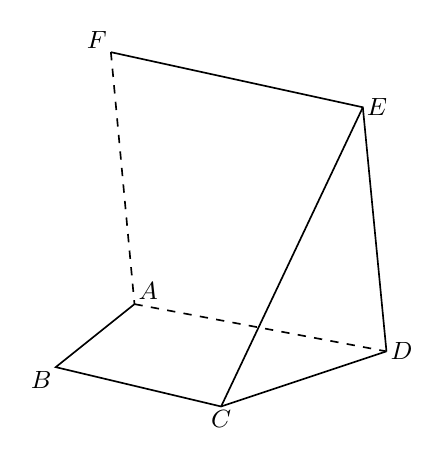
\begin{tikzpicture}[semithick, every node/.style={inner sep=1.2pt, font=\small}]
  \coordinate (F) at (0.2,4.4);
  \coordinate (E) at (3.4,3.7);
  \coordinate (A) at (0.5,1.2);
  \coordinate (D) at (3.7,0.6);
  \coordinate (B) at (-0.5,0.4);
  \coordinate (C) at (1.6,-0.1);
  \draw (F) -- (E) -- (D);
  \draw[dashed] (F) -- (A);
  \draw (A) -- (B) -- (C) -- (D);
  \draw[dashed] (A) -- (D);
  \draw (C) -- (E);
  \node[above left] at (F) {$F$};
  \node[right] at (E) {$E$};
  \node[above right] at (A) {$A$};
  \node[right] at (D) {$D$};
  \node[below left] at (B) {$B$};
  \node[below] at (C) {$C$};
\end{tikzpicture}
\end{center}
\nopagebreak[4]
\Needspace{4\baselineskip}
\textbf{解析}

\Needspace{5\baselineskip}
以 $A$ 为原点，$AD$ 为 $x$ 轴，平面 $ABCD$ 为 $xOy$ 平面建系：

\nopagebreak[4]
\[A(0,0,0),\quad D(2\sqrt2,0,0),\quad F(0,0,2\sqrt2),\quad E(2\sqrt2,0,2\sqrt2).\]

由 $CD=1$、$\angle CDA=45^\circ$ 得 $C\left(\dfrac{3\sqrt2}2,-\dfrac{\sqrt2}2,0\right)$；由 $BC\parallel AD$、$\angle BAD=45^\circ$ 得 $B\left(\dfrac{\sqrt2}2,-\dfrac{\sqrt2}2,0\right)$。

\Needspace{5\baselineskip}
（1）

\nopagebreak[4]
\[\overrightarrow{CE}=\left(\frac{\sqrt2}2,\frac{\sqrt2}2,2\sqrt2\right),\qquad
\overrightarrow{AF}=(0,0,2\sqrt2).\]

\Needspace{5\baselineskip}
故 $|\overrightarrow{CE}|=3$，$|\overrightarrow{AF}|=2\sqrt2$，

\nopagebreak[4]
\[\cos\theta=\frac{\overrightarrow{CE}\cdot\overrightarrow{AF}}{|\overrightarrow{CE}||\overrightarrow{AF}|}
=\frac{8}{6\sqrt2}=\frac{2\sqrt2}3.\]

\Needspace{5\baselineskip}
（2）$\overrightarrow{CD}=\left(\dfrac{\sqrt2}2,\dfrac{\sqrt2}2,0\right)$，而

\nopagebreak[4]
\[\overrightarrow{CD}\cdot\overrightarrow{AB}
=\frac12-\frac12=0,\qquad
\overrightarrow{CD}\cdot\overrightarrow{AF}=0.\]

又 $AB$ 与 $AF$ 是平面 $ABF$ 内两条相交直线，故 $CD\perp$ 平面 $ABF$。

\Needspace{5\baselineskip}
（3）平面 $AEF$ 的法向量可取 $\boldsymbol n_1=(0,1,0)$；平面 $BEF$ 中

\nopagebreak[4]
\[\overrightarrow{EF}=(-2\sqrt2,0,0),\quad
\overrightarrow{EB}=\left(-\frac{3\sqrt2}2,-\frac{\sqrt2}2,-2\sqrt2\right),\]

\Needspace{5\baselineskip}
取 $\boldsymbol n_2=(0,-4,1)$。于是

\nopagebreak[4]
\[\cos\theta=\frac{|\boldsymbol n_1\cdot\boldsymbol n_2|}{|\boldsymbol n_1||\boldsymbol n_2|}
=\frac4{\sqrt{17}},\qquad
\tan\theta=\frac14.\]

\gkanswer{答案：（1）$\dfrac{2\sqrt2}3$；（2）证明；（3）$\dfrac14$。}

\end{answer}
\begin{answer}
\gksolhead{20}{}

\textbf{题目}：

已知函数 $f(x)=ax^3-\dfrac32x^2+1$（$x\in\mathbf R$），其中 $a>0$。

（1）若 $a=1$，求曲线 $y=f(x)$ 在点 $(2,f(2))$ 处的切线方程；

（2）若在区间 $\left[-\dfrac12,\dfrac12\right]$ 上，$f(x)>0$ 恒成立，求 $a$ 的取值范围。

\Needspace{4\baselineskip}
\textbf{解析}

\Needspace{5\baselineskip}
（1）$a=1$ 时 $f(x)=x^3-\dfrac32x^2+1$，$f(2)=3$，$f'(x)=3x^2-3x$，$f'(2)=6$。故切线为

\nopagebreak[4]
\[y-3=6(x-2),\qquad y=6x-9.\]

\Needspace{5\baselineskip}
（2）$f'(x)=3x^2-3x=3x(x-1)$。在 $\left[-\dfrac12,\dfrac12\right]$ 上，$x\in\left(-\dfrac12,0\right)$ 时 $f'>0$，$x\in\left(0,\dfrac12\right)$ 时 $f'<0$，故最小值在端点取得。

\nopagebreak[4]
\[f\left(-\frac12\right)=\frac{5-a}8,\qquad
f\left(\frac12\right)=\frac{a+5}8>0.\]

由 $f\left(-\dfrac12\right)>0$ 得 $a<5$。故 $0<a<5$。

\gkanswer{答案：（1）$y=6x-9$；（2）$0<a<5$。}

\end{answer}
\begin{answer}
\gksolhead{21}{}

\textbf{题目}：

已知椭圆 $\dfrac{x^2}{a^2}+\dfrac{y^2}{b^2}=1$（$a>b>0$）的离心率 $e=\dfrac{\sqrt3}2$，连接椭圆的四个顶点得到的菱形的面积为 $4$。

（1）求椭圆的方程；

（2）设直线 $l$ 与椭圆相交于不同的两点 $A$、$B$，已知点 $A$ 的坐标为 $(-a,0)$。

① 若 $|AB|=\dfrac{4\sqrt2}5$，求直线 $l$ 的倾斜角；

② 若点 $Q(0,y_0)$ 在线段 $AB$ 的垂直平分线上，且 $\overrightarrow{QA}\cdot\overrightarrow{QB}=4$，求 $y_0$ 的值。

\Needspace{4\baselineskip}
\textbf{解析}

\Needspace{5\baselineskip}
（1）四个顶点构成菱形，其面积为 $2ab=4$，故 $ab=2$。又

\nopagebreak[4]
\[e^2=\frac34=1-\frac{b^2}{a^2}\Longrightarrow a=2b.\]

于是 $2b^2=2$，$b=1$，$a=2$，椭圆为 $\dfrac{x^2}4+y^2=1$。

\Needspace{5\baselineskip}
（2）① $A(-2,0)$。设 $l$ 的斜率为 $k$，则 $y=k(x+2)$。代入椭圆得

\nopagebreak[4]
\[(x+2)\left[x-2+4k^2(x+2)\right]=0,\]

\Needspace{5\baselineskip}
另一交点横坐标满足 $x_B+2=\dfrac4{1+4k^2}$，故

\nopagebreak[4]
\[|AB|=\frac{4\sqrt{1+k^2}}{1+4k^2}=\frac{4\sqrt2}5.\]

\Needspace{5\baselineskip}
平方整理得

\nopagebreak[4]
\[32k^4-9k^2-23=0\Longrightarrow(k^2-1)(32k^2+23)=0,\]

故 $k=\pm1$，倾斜角为 $\dfrac\pi4$ 或 $\dfrac{3\pi}4$。

\Needspace{5\baselineskip}
② 由 $Q$ 在 $AB$ 的垂直平分线上得 $|QA|=|QB|$，即

\nopagebreak[4]
\[4+y_0^2=x_B^2+(y_0-y_B)^2
\Longrightarrow 2y_0y_B=x_B^2+y_B^2-4.\]

\Needspace{5\baselineskip}
又 $x_B^2+4y_B^2=4$，故 $x_B^2+y_B^2-4=-3y_B^2$，从而

\nopagebreak[4]
\[y_0=-\frac32y_B.\]

\Needspace{5\baselineskip}
再由 $\overrightarrow{QA}\cdot\overrightarrow{QB}=4$：

\nopagebreak[4]
\[-2x_B-y_0(y_B-y_0)=4
\Longrightarrow -2x_B+\frac{15}4y_B^2=4.\]

\Needspace{5\baselineskip}
与 $x_B^2+4y_B^2=4$ 联立，令 $t=y_B^2$，得

\nopagebreak[4]
\[\left(\frac{15}8t-2\right)^2=4-4t
\Longrightarrow \frac{225}{64}t^2-\frac72t=0
\Longrightarrow t=\frac{224}{225}.\]

故 $y_B=\pm\dfrac{4\sqrt{14}}{15}$，$y_0=-\dfrac32y_B=\mp\dfrac{2\sqrt{14}}5$，即 $y_0=\pm\dfrac{2\sqrt{14}}5$。

\gkanswer{答案：（1）$\dfrac{x^2}4+y^2=1$；（2）① $\dfrac\pi4$ 或 $\dfrac{3\pi}4$；② $\pm\dfrac{2\sqrt{14}}5$。}

\end{answer}
\begin{answer}
\gksolhead{22}{}

\textbf{题目}：

在数列 $\{a_n\}$ 中，$a_1=0$，且对任意 $k\in\mathbf N^*$，$a_{2k-1}$，$a_{2k}$，$a_{2k+1}$ 成等差数列，其公差为 $2k$。

（1）证明 $a_4$，$a_5$，$a_6$ 成等比数列；

（2）求数列 $\{a_n\}$ 的通项公式；

（3）记 $T_n=\dfrac{2^2}{a_2}+\dfrac{3^2}{a_3}+\cdots+\dfrac{n^2}{a_n}$，证明 $\dfrac32<2n-T_n\leqslant2$（$n\geqslant2$）。

\Needspace{4\baselineskip}
\textbf{解析}

\Needspace{5\baselineskip}
（1）由 $a_1=0$ 及公差逐段计算：

\nopagebreak[4]
\[a_2=2,\ a_3=4;\qquad a_4=8,\ a_5=12;\qquad a_6=18.\]

于是 $a_5^2=144=a_4a_6$，故 $a_4,a_5,a_6$ 成等比数列。

\Needspace{5\baselineskip}
（2）由条件

\nopagebreak[4]
\[a_{2k}=a_{2k-1}+2k,\qquad a_{2k+1}=a_{2k}+2k=a_{2k-1}+4k.\]

\Needspace{5\baselineskip}
故奇数项满足 $a_{2k+1}-a_{2k-1}=4k$，累加得

\nopagebreak[4]
\[a_{2k-1}=a_1+\sum_{j=1}^{k-1}4j=2k(k-1);\]

\Needspace{5\baselineskip}
于是

\nopagebreak[4]
\[a_{2k}=a_{2k-1}+2k=2k^2.\]

\Needspace{5\baselineskip}
（3）先算偶、奇项对 $T_n$ 的贡献。对偶数下标 $2k$，

\nopagebreak[4]
\[\frac{(2k)^2}{a_{2k}}=\frac{4k^2}{2k^2}=2;\]

\Needspace{5\baselineskip}
对奇数下标 $2k+1$，

\nopagebreak[4]
\[\frac{(2k+1)^2}{a_{2k+1}}
=\frac{(2k+1)^2}{2k(k+1)}
=2+\frac1{2k(k+1)}.\]

\Needspace{5\baselineskip}
若 $n=2m$，则

\nopagebreak[4]
\[T_{2m}=2m+\sum_{k=1}^{m-1}\left(2+\frac1{2k(k+1)}\right)
=4m-2+\frac12\left(1-\frac1m\right),\]

\Needspace{5\baselineskip}
故

\nopagebreak[4]
\[2n-T_n=4m-T_{2m}=\frac32+\frac1{2m}\in\left(\frac32,2\right].\]

\Needspace{5\baselineskip}
若 $n=2m+1$，同理

\nopagebreak[4]
\[T_{2m+1}=2m+\sum_{k=1}^{m}\left(2+\frac1{2k(k+1)}\right)
=4m+\frac12\left(1-\frac1{m+1}\right),\]

\Needspace{5\baselineskip}
故

\nopagebreak[4]
\[2n-T_n=4m+2-T_{2m+1}
=\frac32+\frac1{2(m+1)}\in\left(\frac32,2\right].\]

综上，$\dfrac32<2n-T_n\leqslant2$（$n\geqslant2$）。

\gkanswer{答案：（1）证明；（2）$a_{2k}=2k^2$，$a_{2k-1}=2(k-1)k$；（3）证明。}

\end{answer}